
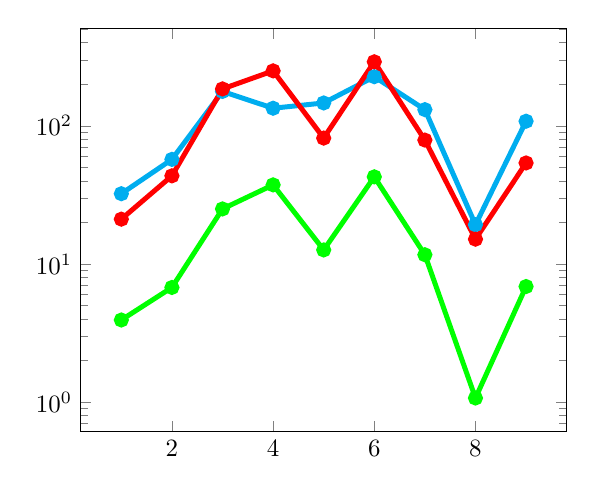
\begin{tikzpicture}[scale=0.9]
\begin{semilogyaxis}
\addplot[mark=*,color=cyan,line width=2pt,mark options={solid}] coordinates {(1,32.244785)(2,57.142866)(3,177.300524)(4,133.978037)(5,146.279183)(6,226.548281)(7,130.892825)(8,19.238491)(9,107.901228)};
\addplot[mark=*,color=red,line width=2pt,mark options={solid}] coordinates {(1,21.105355)(2,43.435309)(3,184.89286)(4,249.706248)(5,81.458676)(6,290.469176)(7,78.83509)(8,15.117246)(9,53.835425)};
\addplot[mark=*,color=green,line width=2pt,mark options={solid}] coordinates {(1,3.933221)(2,6.762879)(3,25.027742)(4,37.363271)(5,12.63568)(6,42.715093)(7,11.664699)(8,1.07143)(9,6.86998)};

\end{semilogyaxis}
\end{tikzpicture}
